
\section{Digimode per SSB}
\label{section:digimode_ssb}
\begin{frame}%STARTCONTENT

\frametitle{Bandbreite von Digimodes}
\begin{itemize}
  \item Im Gegensatz zur Sprache benötigen viele Digimodes weniger Bandbreite
  \item Z.B. BPSK31 mit \qty{31,25}{\hertz} oder FT8 mit \qty{50}{\hertz}
  \item Die erzeugten Töne werden mittels Kurzwelle in SSB moduliert
  \item Die Bandbreite des ausgestrahlten Signals bleibt dabei gleich
  \end{itemize}
\end{frame}

\begin{frame}
\only<1>{
\begin{QQuestion}{EE403}{Bei der Aussendung eines digitalen Signals mittels eines Funkgerätes in SSB-Einstellung beträgt die NF-Bandbreite des in das Funkgerät eingespeisten Signals \qty{50}{\Hz}. Wie groß ist die HF-Bandbreite?}{$\sqrt{2} \cdot$ \qty{50}{\Hz}}
{\qty{100}{\Hz}}
{\qty{25}{\Hz}}
{\qty{50}{\Hz}}
\end{QQuestion}

}
\only<2>{
\begin{QQuestion}{EE403}{Bei der Aussendung eines digitalen Signals mittels eines Funkgerätes in SSB-Einstellung beträgt die NF-Bandbreite des in das Funkgerät eingespeisten Signals \qty{50}{\Hz}. Wie groß ist die HF-Bandbreite?}{$\sqrt{2} \cdot$ \qty{50}{\Hz}}
{\qty{100}{\Hz}}
{\qty{25}{\Hz}}
{\textbf{\textcolor{DARCgreen}{\qty{50}{\Hz}}}}
\end{QQuestion}

}
\end{frame}

\begin{frame}
\only<1>{
\begin{QQuestion}{EE402}{Welche Modulation wird am Transceiver eingestellt, um ein schmalbandiges digitales Signal (z.~B. BPSK31 oder FT8), das per Audiosignal als NF eingespeist wird, unter Beibehaltung der Bandbreite in HF umzusetzen?}{Phasenmodulation (PM)}
{Frequenzmodulation (FM)}
{Amplitudenmodulation (AM)}
{Einseitenbandmodulation (SSB)}
\end{QQuestion}

}
\only<2>{
\begin{QQuestion}{EE402}{Welche Modulation wird am Transceiver eingestellt, um ein schmalbandiges digitales Signal (z.~B. BPSK31 oder FT8), das per Audiosignal als NF eingespeist wird, unter Beibehaltung der Bandbreite in HF umzusetzen?}{Phasenmodulation (PM)}
{Frequenzmodulation (FM)}
{Amplitudenmodulation (AM)}
{\textbf{\textcolor{DARCgreen}{Einseitenbandmodulation (SSB)}}}
\end{QQuestion}

}
\end{frame}

\begin{frame}
\frametitle{Empfang von Digimodes}
\begin{columns}
    \begin{column}{0.48\textwidth}
    \begin{itemize}
  \item Beim Empfang von SSB können in der üblichen Bandbreite von \qty{2,4}{\kilo\hertz} mehrere schmalbandige Digimodes empfangen werden
  \item FT8: \qty{2400}{\hertz}  $\div$  \qty{50}{\hertz} = max. 48 Signale
  \item BPSK31: \qty{2400}{\hertz}  $\div$  \qty{31,25}{\hertz} = max. 76 Signale
  \item Am Computer wird dann das gewünschte Digimode-Signal selektiert
  \end{itemize}

    \end{column}
   \begin{column}{0.48\textwidth}
       
\begin{figure}
    \DARCimage{0.85\linewidth}{718include}
    \caption{\scriptsize Wasserfalldiagramm vom Empfang von mehreren Digimode-Signalen innerhalb der SSB-Bandbreite von \qty{2,4}{\kilo\hertz}. Jede Spalte ist die Übertragung eines anderen Signals}
    \label{e_digimode_ssb_ft8_wasserfall}
\end{figure}


   \end{column}
\end{columns}

\end{frame}

\begin{frame}
\only<1>{
\begin{QQuestion}{EE404}{Wie viele digitale Signale unterschiedlicher Stationen können mit einem analogen Funkgerät (\qty{2,4}{\kHz} SSB-Bandbreite) und einem über die Audio-Schnittstelle angeschlossenen Computer gleichzeitig empfangen und dekodiert werden?}{Es können je nach Art der Signale ein oder mehrere Signale empfangen werden.}
{Es können maximal zwei Signale empfangen werden (eines pro Seitenband).}
{Es kann maximal ein Signal empfangen werden, da ein Seitenband genutzt wird.}
{Es kann maximal ein Signal empfangen werden, außer das Funkgerät verfügt über doppelte Kanalbandbreite.}
\end{QQuestion}

}
\only<2>{
\begin{QQuestion}{EE404}{Wie viele digitale Signale unterschiedlicher Stationen können mit einem analogen Funkgerät (\qty{2,4}{\kHz} SSB-Bandbreite) und einem über die Audio-Schnittstelle angeschlossenen Computer gleichzeitig empfangen und dekodiert werden?}{\textbf{\textcolor{DARCgreen}{Es können je nach Art der Signale ein oder mehrere Signale empfangen werden.}}}
{Es können maximal zwei Signale empfangen werden (eines pro Seitenband).}
{Es kann maximal ein Signal empfangen werden, da ein Seitenband genutzt wird.}
{Es kann maximal ein Signal empfangen werden, außer das Funkgerät verfügt über doppelte Kanalbandbreite.}
\end{QQuestion}

}
\end{frame}

\begin{frame}
\frametitle{SSTV}
\begin{columns}
    \begin{column}{0.48\textwidth}
    \begin{itemize}
  \item \emph{Slow-Scan Television} ist die Übertragung von Standbildern mittels Digimodes
  \item Zeilenweise Übertragung von Bildern
  \item Verschiedene Verfahren mit verschiedenen Auflösungen und Übertragungsgeschwindigkeiten
  \item Bandbreite unter 3kHz und in Kurzwellenbändern nutzbar
  \end{itemize}

    \end{column}
   \begin{column}{0.48\textwidth}
       
\begin{figure}
    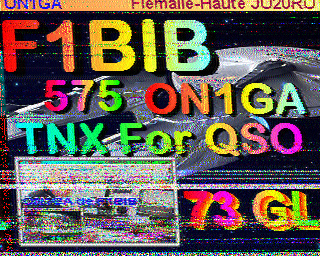
\includegraphics[width=0.85\textwidth]{foto/84}
    \caption{\scriptsize Bestätigung einer SSTV Verbindung an F1BIB von ON1GA mit dem RST 575 und zusätzlich dem ursprünglich empfangenen Bild}
    \label{e_digimode_ssb_sstv}
\end{figure}

   \end{column}
\end{columns}

\end{frame}

\begin{frame}
\frametitle{ATV}
\begin{itemize}
  \item \emph{Amateur Television} ist die Übertragung von Bewegtbildern
  \item Benötigt mehrere MHz Bandbreite (\qty{6}{\mega\hertz} und mehr)
  \item Deshalb nur ab \qty{70}{\centi\metre} Band aufwärts nutzbar
  \end{itemize}
\end{frame}

\begin{frame}
\only<1>{
\begin{QQuestion}{EE415}{Welcher Unterschied zwischen ATV und SSTV ist richtig?}{SSTV wird nur auf Kurzwelle, ATV auf UKW verwendet.}
{SSTV überträgt Standbilder, ATV bewegte Bilder.}
{SSTV belegt eine größere Bandbreite als ATV.}
{SSTV ist schwarzweiß, ATV in Farbe.}
\end{QQuestion}

}
\only<2>{
\begin{QQuestion}{EE415}{Welcher Unterschied zwischen ATV und SSTV ist richtig?}{SSTV wird nur auf Kurzwelle, ATV auf UKW verwendet.}
{\textbf{\textcolor{DARCgreen}{SSTV überträgt Standbilder, ATV bewegte Bilder.}}}
{SSTV belegt eine größere Bandbreite als ATV.}
{SSTV ist schwarzweiß, ATV in Farbe.}
\end{QQuestion}

}
\end{frame}%ENDCONTENT
